%
% Comparaciones de desempeño de la API.
% Implementación de de la API web, reporte técnico.
%
% Proyecto Lovelace.
%

\section{Resultados}
\label{sec:resultados_api}

\subsection{Desempeño de la \texorpdfstring{\acrshort{gl:api}}{API}}
\label{sec:comparacion_api}

Con la finalidad de probar el desempeño de la \gls{gl:api} desarrollada, se
hizo la medición del los tiempo de respuesta de las peticiones de operaciones
de tokenización y detokenización con los 5 métodos disponibles.

En la tabla~\ref{tabla:tiempos_peticiones_tokenizacion} se pueden observar
los tiempos obtenidos de las pruebas de desempeño de la \gls{gl:api}, los
cuales se obtuvieron al realizar 10K peticiones de operaciones de
tokenización y detokenización con cada método posible.

\begin{table}
  \begin{center}
    \begin{tabular}{c|c|c|}
      \cline{2-3}
      & Tokenización & Detokenización \\
      \hline
      \multicolumn{1}{|c|}{\acrshort{gl:ffx}}
        & 206.526 s & 208.204 s \\\hline
      \multicolumn{1}{|c|}{\acrshort{gl:bps}}
        & 219.036 s & 219.448 s \\\hline
      \multicolumn{1}{|c|}{TKR}
        & 824.969 s & 103.854 s \\\hline
      \multicolumn{1}{|c|}{AHR}
        & 436.053 s & 132.297 s \\\hline
      \multicolumn{1}{|c|}{\acrshort{gl:drbg}}
        & 437.406 s & 124.064 s \\\hline
    \end{tabular}
    \caption{Comparación de tiempos.}
    \label{tabla:tiempos_peticiones_tokenizacion}
  \end{center}
\end{table}


Con los datos de la tabla~\ref{tabla:tiempos_peticiones_tokenizacion} se generó
la gráfica de la figura~\ref{figura:peticiones_tokenizacion_grafica} donde se
puede ver de forma más clara la diferencia en los tiempos.

\begin{figure}
  \begin{center}
    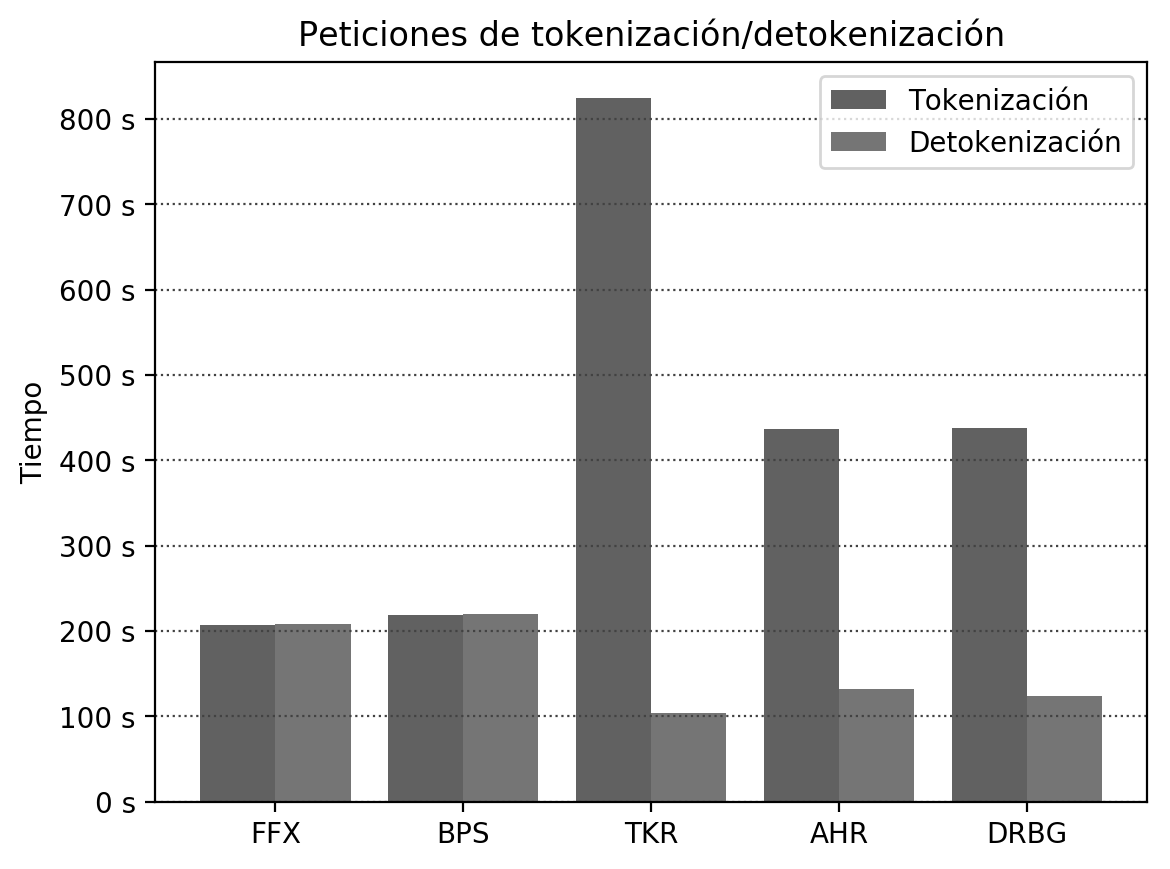
\includegraphics[width=0.7\linewidth]
      {diagramas/peticiones_tokenizacion_grafica}
  \end{center}
  \caption{Comparación de tiempos de operación.}
  \label{figura:peticiones_tokenizacion_grafica}
\end{figure}
